%------------------------------------------------------------------------
%Editar Diplomado
\hypertarget{cv:eliminarPExt}{\section{Eliminar Puntos de Extensión}} \label{sec:eliminarPExt}

	Esta funcionalidad le permitirá eliminar un punto de extensión innecesario o incorrecto. 

		\subsection{Procedimiento}

			%Pasos de procedimiento
			\begin{enumerate}
	
			\item Oprima el botón \IUBotonEliminar{} de un registro existente de la pantalla \ref{fig:GestionarPuntosExt} ''Gestionar Puntos de Extensión''.
	
			\item Se mostrará el mensaje \ref{fig:confirmaEliminaPExt} sobre la pantalla \ref{fig:GestionarPuntosExt} ''Gestionar Puntos de Extensión''.
			
			%Pantalla
			\begin{figure}[htbp!]
				\begin{center}
					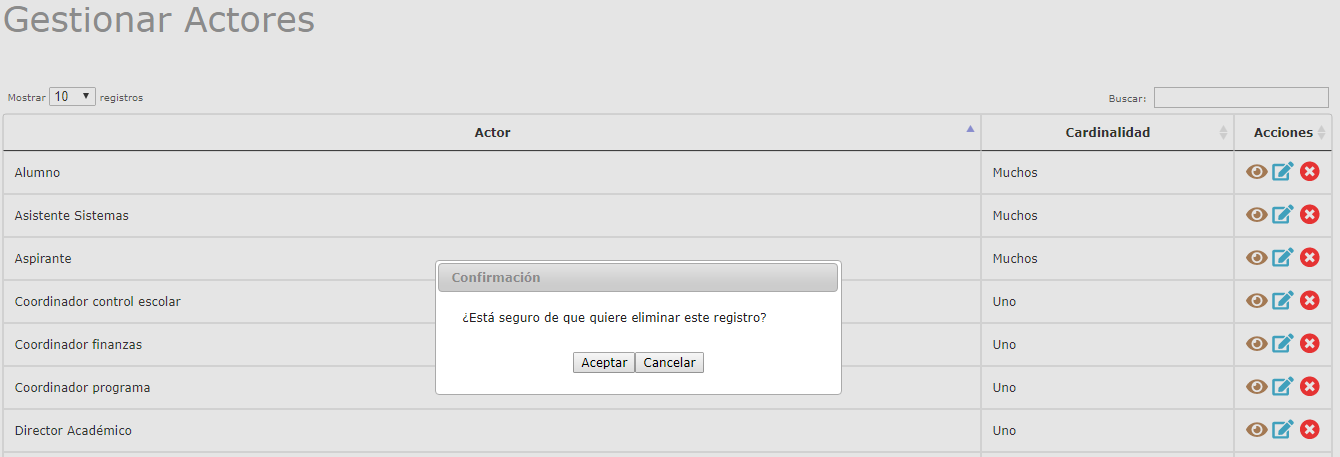
\includegraphics[scale=0.5]{roles/lider/actor/pantallas/IU10-3MSG10}
					\caption{MSG de Confirmación}
					\label{fig:confirmaEliminaPExt}
				\end{center}
			\end{figure}
						
			\item Oprima el botón \IUAceptar.
			
			\item Se mostrará el mensaje \ref{fig:PExtEliminado} en la pantalla \ref{fig:GestionarPuntosExt} ''Gestionar Puntos de Extensión''.
			
			\begin{figure}[htbp!]
				\begin{center}
					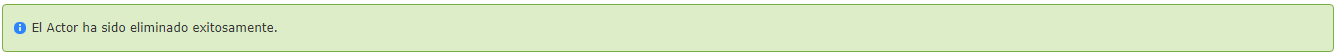
\includegraphics[scale=0.5]{roles/lider/actor/pantallas/IU10-3MSG1}
					\caption{MSG: Punto de extensión Eliminado}
					\label{fig:PExtEliminado}
				\end{center}
			\end{figure}
			\end{enumerate}